\documentclass[12pt]{report}
\usepackage[utf8]{inputenc}
\usepackage[T1]{fontenc}
\usepackage{lmodern}
\usepackage[margin=2.5cm]{geometry}
\usepackage{graphicx}
\usepackage{listings}
\usepackage{color}
\usepackage{hyperref}
\usepackage{float}
\usepackage{titlesec}
\usepackage{setspace}
\usepackage{fancyhdr}
\usepackage{array}
\usepackage{enumitem}
\usepackage{tcolorbox}
\usepackage{minted}
\usepackage{times}
\usepackage{tabularx}
\usepackage{booktabs}
\usepackage{xcolor}

% Format headings
\titleformat{\chapter}{\normalfont\fontsize{16}{19}\bfseries}{\thechapter}{1em}{}
\titleformat{\section}{\normalfont\fontsize{14}{17}\bfseries}{\thesection}{1em}{}
\titleformat{\subsection}{\normalfont\fontsize{12}{15}\bfseries}{\thesubsection}{1em}{}

% Set normal text size to 12pt
\renewcommand{\normalsize}{\fontsize{12}{14}\selectfont}

\geometry{
    a4paper,
    margin=2.5cm
}

% Code styling
\definecolor{codegreen}{rgb}{0,0.6,0}
\definecolor{codegray}{rgb}{0.5,0.5,0.5}
\definecolor{codepurple}{rgb}{0.58,0,0.82}
\definecolor{backcolour}{rgb}{0.95,0.95,0.92}

\lstdefinestyle{mystyle}{
    backgroundcolor=\color{backcolour},   
    commentstyle=\color{codegreen},
    keywordstyle=\color{magenta},
    numberstyle=\tiny\color{codegray},
    stringstyle=\color{codepurple},
    basicstyle=\ttfamily\footnotesize,
    breakatwhitespace=false,         
    breaklines=true,                 
    captionpos=b,                    
    keepspaces=true,                 
    numbers=left,                    
    numbersep=5pt,                  
    showspaces=false,                
    showstringspaces=false,
    showtabs=false,                  
    tabsize=2
}

\lstset{style=mystyle}

% Setup fancy header and footer
\pagestyle{fancy}
\fancyhead{}
\fancyfoot{}
\fancyhead[L]{HealthHub}
\fancyhead[R]{\thepage}
\fancyfoot[C]{RV College of Engineering}
\renewcommand{\headrulewidth}{2pt}
\renewcommand{\footrulewidth}{1pt}

% Title page formatting
\renewcommand{\maketitle}{
    \begin{titlepage}
        \centering
        \vspace*{-1cm}
        
        % Logo and College Name
        \includegraphics[width=0.2\textwidth]{images/rvce_logo.jpeg}\par\vspace{0.5cm}
        {\huge\bfseries RV College of Engineering®\par}
        \vspace{0.5cm}
        {\Large Go, change the world\par}
        \vspace{1cm}
        
        
        % Lab Report Title
        {\Large\bfseries Final Experiental Learning Report\par}
        \vspace{0.5cm}
        
        % Title
        {\Large\bfseries HEALTHHUB: A COMPREHENSIVE HEALTH\\
        DATA MANAGEMENT PLATFORM\par}
        \vspace{1.5cm}
        
        % Submitted by
        {\large\bfseries Submitted by\par}
        \vspace{0.5cm}
        \begin{tabular}{ll}
            Ansh Ravi Kashyap & USN: 1RV23CS040 \\
            Ashwin Nagendra Bhat & USN: 1RV23CS055 \\
            Avinash Anish & USN: 1RV23IS145 \\
            Aarnav Kembhavi & USN: 1RV23CS309 \\
            Vishal Joy & USN: 1RV23CD059
            
            
        \end{tabular}
        \vspace{1.5cm}
        
        
        % Academic Year
        {\large 2024-2025}
    \end{titlepage}
}

\title{\fontsize{16}{19}\selectfont HealthHub: A Comprehensive Health Data Management Platform\\
       Implementation and Analysis Report}
\author{Department of Information Science and Engineering\\
        RV College of Engineering}
\date{\today}

\begin{document}

\maketitle

\tableofcontents
\newpage

% Abstract
\begin{abstract}
This paper presents HealthHub, an AI-powered personal health assistant designed to help individuals make informed daily dietary choices by providing personalized food safety and nutritional insights. Users can log food intake, which HealthHub analyzes using a Retrieval-Augmented Generation (RAG) pipeline to query diverse sources like FSSAI advisories and food databases, and an SQL agent for nutritional pattern analysis. The system uniquely integrates personal health sensor data (e.g., heart rate) to correlate diet with physiological responses, offering potential risk warnings. HealthHub features an intuitive voice and video-enabled interface, aiming to empower users with accessible, actionable information for enhanced food safety awareness and personal well-being. Performance evaluations highlight the system's capability in processing user queries effectively and integrating multimodal data for comprehensive dietary support.
\end{abstract} 

% CHAPTER 1: INTRODUCTION
\chapter{INTRODUCTION}
% Chapter 1: Introduction to IoT-Based Vital Sign Monitoring System with Conversational Health Data Access
% This section should contain the use of the project in real time, as per the provided guidelines.

\section*{Introduction}
Your introduction content goes here.
      % Introduction
\section{PROBLEM STATEMENT}

As shown in Figure \ref{fig:problem-definition}, the healthcare industry faces significant challenges in managing and utilizing personal health data effectively:

\begin{figure}[H]
    \centering
    \includegraphics[width=0.8\textwidth]{images/problem-definition.png}
    \caption{Problem Definition Overview}
    \label{fig:problem-definition}
\end{figure}

\subsection{Why this project is being created}
\begin{itemize}
    \item To address the growing complexity of managing personal health information
    \item To provide a unified health monitoring solution that integrates various data sources and offers intelligent insights
\end{itemize}

\subsection{Problems or needs this software addresses}
\begin{itemize}
    \item The challenge of consolidating and managing disparate health data from different sources
    \item The need for real-time sensor monitoring and personalized health insights
    \item The demand for advanced AI-powered analysis to support better health management
\end{itemize}

\subsection{Functionalities this software will include}
\begin{itemize}
    \item Integration of real-time sensor data, health records, and nutrition logs
    \item Implementation of a RAG (Retrieval-Augmented Generation) pipeline for intelligent data processing
    \item Delivery of personalized health insights through AI-powered analysis
    \item Use of advanced technologies like LangChain, OpenAI's GPT models, and vector databases for contextual information retrieval and analysis
\end{itemize}  % Problem Statement
\section{OBJECTIVES}

\begin{enumerate}
    \item \textbf{To Build an IoT Health Monitoring System}
    \begin{itemize}
        \item Set up Arduino-based sensors for ECG, heart rate, pulse, and temperature monitoring
        \item Create a system to collect real-time vital sign data
        \item Design a dashboard to display live health measurements
    \end{itemize}

    \item \textbf{To Create a Natural Language Interface}
    \begin{itemize}
        \item Develop a conversational system using LLM models
        \item Enable users to ask questions about their health data in simple language
        \item Provide easy-to-understand responses to health data queries
    \end{itemize}

    \item \textbf{To Make Health Data Easy to Understand}
    \begin{itemize}
        \item Convert complex health readings into simple explanations
        \item Create visual representations of health trends
        \item Provide personalized health insights based on collected data
    \end{itemize}

    \item \textbf{To Ensure Data Safety and Privacy}
    \begin{itemize}
        \item Protect user health data through encryption
        \item Follow healthcare data protection rules
        \item Create secure ways to store and access health information
    \end{itemize}
\end{enumerate}        % Objectives

% CHAPTER 2: LITERATURE SURVEY
\chapter{LITERATURE SURVEY}
\section{IoT-Based Health Monitoring Systems}

\begin{enumerate}
    \item Remote Patient Monitoring Systems
    \begin{itemize}
        \item Commercial solutions like Philips HealthSuite Digital Platform and Medtronic CareLink provide continuous monitoring but typically lack conversational interfaces
        \item Most systems require healthcare provider interpretation of data
        \item Limited personalization capabilities for individual user needs
    \end{itemize}

    \item Wearable Health Trackers
    \begin{itemize}
        \item Consumer devices (Fitbit, Apple Watch, Samsung Galaxy Watch) offer basic vital sign monitoring
        \item Typically monitor limited parameters (heart rate, activity, sometimes ECG)
        \item Data presentation is primarily visual/graphical with minimal natural language interpretation
        \item Users often struggle to contextualize the health significance of their data
    \end{itemize}

    \item Smart Home Health Monitoring
    \begin{itemize}
        \item Smart home platforms integrating health devices (Amazon Alexa + Omron blood pressure monitor)
        \item Basic voice command capabilities but limited to simple queries
        \item Lack comprehensive vital sign integration and contextual health understanding
    \end{itemize}
\end{enumerate}

\section{Conversational Health Interfaces}

\begin{enumerate}
    \item Healthcare Chatbots
    \begin{itemize}
        \item Systems like Ada Health, Babylon Health, and Buoy Health provide symptom assessment
        \item Focus primarily on diagnostic information rather than personal health data interpretation
        \item Limited integration with real-time physiological monitoring devices
        \item Typically use rule-based approaches rather than advanced NLP techniques
    \end{itemize}

    \item Voice Assistants in Healthcare
    \begin{itemize}
        \item Voice-enabled systems (Alexa Skills for healthcare, Google Assistant healthcare actions)
        \item Capabilities include medication reminders, appointment scheduling, and basic health information
        \item Limited in processing and contextualizing continuous health data streams
        \item Privacy concerns with cloud-based processing of sensitive health information
    \end{itemize}

    \item Natural Language Understanding in Health Data
    \begin{itemize}
        \item Research systems employing NLP for electronic health records (EHRs)
        \item Focus on clinical documentation rather than consumer-facing applications
        \item Limited capabilities for real-time data processing from IoT devices
        \item Few systems combine IoT sensor data with conversational interfaces
    \end{itemize}
\end{enumerate}

\section{Key Limitations}

\begin{enumerate}
    \item Integration Challenges
    \begin{itemize}
        \item Most solutions either focus on robust IoT monitoring OR natural language interfaces, rarely both
        \item Limited interconnectivity between sensing devices and conversational systems
        \item Data silos prevent comprehensive health insights
    \end{itemize}

    \item Technical Complexity
    \begin{itemize}
        \item Existing systems often require technical expertise to install, configure and interpret
        \item Complex user interfaces create barriers for elderly or non-technical users
        \item Data visualization without context-aware explanations limits usefulness
    \end{itemize}

    \item Limited Personalization
    \begin{itemize}
        \item Generic health advice rather than personalized insights based on individual data patterns
        \item Minimal adaptation to user's health literacy level or communication preferences
        \item One-size-fits-all approaches to data presentation and interaction
    \end{itemize}

    \item Privacy and Security
    \begin{itemize}
        \item Centralized data storage raising privacy issues
        \item Limited transparency in how health data is processed and stored
        \item Inadequate security measures for sensitive personal health information
    \end{itemize}

    \item RAG Limitations
    \begin{itemize}
        \item Few systems leverage RAG capabilities for personalized health information retrieval
        \item Limited contextual understanding when processing natural language queries about health data
        \item Lack of integration between personal health data repositories and language models
    \end{itemize}
\end{enumerate}

\begin{figure}[h!]
    \centering
    \includegraphics[width=\textwidth]{images/lr2.png}
    \caption{Literature review comparison of existing systems (Part 1)}
\end{figure}

\begin{figure}[h!]
    \centering
    \includegraphics[width=\textwidth]{images/lr3.png}
    \caption{Literature review comparison of existing systems (Part 2)}
\end{figure}  % All literature review content

% CHAPTER 3: DESIGN
\chapter{DESIGN}
\section{METHODOLOGY}

\subsection{Implementation Tasks}

\begin{enumerate}

\item \textbf{Frontend Development}
\begin{itemize}
    \item Design the user interface using \textbf{Next.js} with \textbf{TailwindCSS} and \textbf{shadcn/ui} for a responsive, modular experience.
    \item Build a real-time dashboard to visualize health metrics such as SpO2, heart rate, ECG, and temperature.
    \item Integrate Supabase Auth to enable secure user login and session handling.
\end{itemize}

\item \textbf{Backend Development}
\begin{itemize}
    \item Set up a \textbf{FastAPI} server to handle incoming sensor data and expose RESTful endpoints.
    \item Use a \textbf{PostgreSQL} database (hosted via Supabase) to store and manage health data securely.
    \item Develop APIs for data submission, retrieval, and query handling.
\end{itemize}

\item \textbf{IoT Sensor Integration}
\begin{itemize}
    \item Use an \textbf{Arduino UNO R3} to interface with all biomedical sensors and read analog/digital inputs.
    \item Employ an \textbf{ESP8266 Wi-Fi module} to transmit data to the cloud via HTTP or MQTT.
    \item Configure periodic data sampling and preprocessing before cloud transmission.
\end{itemize}

\item \textbf{AI Integration}
\begin{itemize}
    \item Integrate a conversational AI interface using \textbf{LangChain} and \textbf{GPT-4/GPT-4o}.
    \item Allow users to query their health records through natural language using a Text-to-SQL pipeline.
    \item Provide automated health summaries and anomaly detection powered by AI.
\end{itemize}

\end{enumerate}
       % System Architecture & Flow Diagrams
\section{System Design and Implementation}

\subsection{Requirements Specification}

\subsubsection{Functional Requirements}
\begin{enumerate}
    \item \textbf{Health Data Management}
    \begin{itemize}
        \item Upload and process medical records
        \item Store and retrieve health data securely
        \item Manage user health profiles
    \end{itemize}

    \item \textbf{AI-Powered Chat System}
    \begin{itemize}
        \item Process natural language queries
        \item Provide context-aware responses
        \item Access and utilize medical knowledge base
    \end{itemize}

    \item \textbf{Real-time Health Monitoring}
    \begin{itemize}
        \item Collect sensor data (heart rate, temperature, SpO2)
        \item Display real-time health metrics
        \item Store historical health data
    \end{itemize}
\end{enumerate}

\subsubsection{Non-Functional Requirements}
\begin{enumerate}
    \item \textbf{Performance}
    \begin{itemize}
        \item Response time < 2 seconds for queries
        \item Real-time data updates < 100ms
        \item Support multiple concurrent users
    \end{itemize}

    \item \textbf{Security}
    \begin{itemize}
        \item Secure data transmission
        \item User authentication and authorization
        \item HIPAA compliance considerations
    \end{itemize}

    \item \textbf{Reliability}
    \begin{itemize}
        \item System availability > 99.9%
        \item Data backup and recovery
        \item Error handling and logging
    \end{itemize}
\end{enumerate}

\subsection{System Architecture}
The system follows a modern microservices architecture:

\begin{enumerate}
    \item \textbf{Frontend Layer}
    \begin{itemize}
        \item Next.js 14 application with App Router
        \item TypeScript for type safety
        \item Tailwind CSS and shadcn/ui for UI components
        \item TanStack Query for data fetching
    \end{itemize}

    \item \textbf{Backend Services}
    \begin{itemize}
        \item FastAPI service for RAG pipeline
        \item Supabase for real-time data and authentication
        \item PostgreSQL with pgvector for vector storage
    \end{itemize}

    \item \textbf{External Services}
    \begin{itemize}
        \item Cohere for embedding generation
        \item Arduino IoT platform for sensor data
    \end{itemize}
\end{enumerate}

\subsection{RAG Implementation}
The RAG pipeline is implemented as follows:

\begin{enumerate}
    \item \textbf{Document Processing}
    \begin{itemize}
        \item Medical records are uploaded and processed
        \item Text is extracted and chunked
        \item Cohere generates embeddings
        \item Vectors stored in Supabase pgvector
    \end{itemize}

    \item \textbf{Query Processing}
    \begin{itemize}
        \item User queries processed through Next.js API
        \item FastAPI backend handles embedding generation
        \item Vector similarity search retrieves context
        \item Response generated using retrieved context
    \end{itemize}
\end{enumerate}

\subsection{Real-time Health Monitoring}
The health monitoring system consists of:

\begin{enumerate}
    \item \textbf{Hardware Layer}
    \begin{itemize}
        \item Arduino UNO with ESP8266 WiFi module
        \item Multiple health sensors (Heart rate, Temperature, SpO2)
        \item Real-time data transmission setup
    \end{itemize}

    \item \textbf{Data Integration}
    \begin{itemize}
        \item Supabase real-time subscriptions
        \item Live data visualization using Recharts
        \item Automatic data synchronization
    \end{itemize}
\end{enumerate}

\begin{figure}[H]
    \centering
    \includegraphics[width=0.8\textwidth]{images/system_architecture.png}
    \caption{Overall System Architecture}
\end{figure}

\subsection{Key Features Implementation}

\subsubsection{Health Data Management}
\begin{itemize}
    \item Secure medical record storage
    \item Real-time sensor data integration
    \item Historical data analysis
\end{itemize}

\subsubsection{AI-Powered Chat}
\begin{itemize}
    \item Context-aware responses
    \item Medical knowledge integration
    \item Personalized health insights
\end{itemize}

\subsubsection{Real-time Monitoring}
\begin{itemize}
    \item Live health metrics visualization
    \item Automated data collection
    \item Trend analysis and reporting
\end{itemize}

\begin{figure}[H]
    \centering
    \includegraphics[width=0.8\textwidth]{images/feature_implementation.png}
    \caption{Feature Implementation Overview}
\end{figure}

\subsection{Implementation Details}

\subsubsection{Frontend Components}
Example of a React component using TanStack Query:
\begin{lstlisting}[language=typescript,
                   basicstyle=\ttfamily\small,
                   keywordstyle=\color{blue},
                   stringstyle=\color{red},
                   commentstyle=\color{green!60!black}]
// app/health-records/page.tsx
export default function HealthRecords() {
    const { data, isLoading } = useQuery({
        queryKey: ['health-records'],
        queryFn: fetchHealthRecords,
    })

    if (isLoading) return <LoadingSpinner />

    return (
        <div className="grid grid-cols-1 md:grid-cols-2 gap-4">
            {data?.map((record) => (
                <RecordCard key={record.id} record={record} />
            ))}
        </div>
    )
}
\end{lstlisting}

\subsubsection{Backend Services}
Example of FastAPI endpoint and vector search:
\begin{lstlisting}[language=python,
                   basicstyle=\ttfamily\small,
                   keywordstyle=\color{blue},
                   stringstyle=\color{red},
                   commentstyle=\color{green!60!black}]
@router.post("/rag-query")
async def rag_query(request: RAGQueryRequest):
    try:
        query_embedding = generate_embedding(request.query)
        search_results = query_embeddings(query_embedding)
        context = "\n".join([
            result['text_content'] 
            for result in search_results
        ])
        return {
            "query": request.query,
            "context": context,
            "response": f"Response based on context: {context}"
        }
    except Exception as e:
        raise HTTPException(status_code=500, detail=str(e))
\end{lstlisting}

\subsubsection{Vector Search Implementation}
PostgreSQL function for vector similarity search:
\begin{lstlisting}[language=sql,
                   basicstyle=\ttfamily\small,
                   keywordstyle=\color{blue},
                   stringstyle=\color{red},
                   commentstyle=\color{green!60!black}]
CREATE OR REPLACE FUNCTION match_documents (
    query_embedding vector(1536),
    match_threshold float,
    match_count int
)
RETURNS TABLE (
    id bigint,
    content text,
    similarity float
)
LANGUAGE plpgsql
AS $$
BEGIN
    RETURN QUERY
    SELECT
        documents.id,
        documents.content,
        1 - (documents.embedding <=> query_embedding) AS similarity
    FROM documents
    WHERE 1 - (documents.embedding <=> query_embedding) > match_threshold
    ORDER BY similarity DESC
    LIMIT match_count;
END;
$$;
\end{lstlisting}

\subsubsection{RAG Pipeline Implementation}
The RAG system is implemented through a Next.js API route that communicates with our FastAPI backend:

\begin{lstlisting}[language=typescript,
                   basicstyle=\ttfamily\small,
                   keywordstyle=\color{blue},
                   stringstyle=\color{red},
                   commentstyle=\color{green!60!black}]
// app/api/rag-query/route.ts
export async function POST(req: NextRequest) {
  const body = await req.json();
  const { query, llm_choice, match_count, user_id } = body;

  try {
    const response = await fetch(`${API_URL}/rag-query-v2`, {
      method: 'POST',
      headers: {
        'Content-Type': 'application/json',
      },
      body: JSON.stringify({ 
        query, 
        llm_choice, 
        match_count, 
        user_id
      }),
    });

    if (!response.ok) {
      throw new Error('Failed to get response from RAG query');
    }

    const data = await response.json();
    return NextResponse.json(data);
  } catch (error) {
    return NextResponse.json(
      { error: 'An error occurred during the RAG query' }, 
      { status: 500 }
    );
  }
}
\end{lstlisting}

\subsubsection{Real-time Health Monitoring}
The health monitoring dashboard implements real-time data visualization using Supabase subscriptions:

\begin{lstlisting}[language=typescript,
                   basicstyle=\ttfamily\small,
                   keywordstyle=\color{blue},
                   stringstyle=\color{red},
                   commentstyle=\color{green!60!black}]
// app/(app)/health/monitor/page.tsx
export default function HealthMonitor() {
  const [healthData, setHealthData] = useState<HealthData[]>([]);
  const [isStreaming, setIsStreaming] = useState(false);
  const supabase = createSupabaseBrowser();

  useEffect(() => {
    const channel = supabase
      .channel('sensor_data')
      .on(
        'postgres_changes',
        {
          event: 'INSERT',
          schema: 'public',
          table: 'sensor_data',
        },
        (payload) => {
          if (isStreaming) {
            setHealthData(prevData => {
              const newData = [...prevData, payload.new as HealthData];
              return newData.slice(-100); // Keep last 100 records
            });
          }
        }
      )
      .subscribe();

    return () => {
      supabase.removeChannel(channel);
    };
  }, [supabase, isStreaming]);

  return (
    <div className="grid grid-cols-1 md:grid-cols-2 gap-4">
      <HealthChart 
        data={healthData} 
        dataKey="beat_avg" 
        title="Heart Rate" 
        unit="bpm" 
        chartType={chartType} 
      />
      {/* Other charts */}
    </div>
  );
}
\end{lstlisting}

\subsubsection{Health Data Visualization}
Implementation of the chart component for health metrics:

\begin{lstlisting}[language=typescript,
                   basicstyle=\ttfamily\small,
                   keywordstyle=\color{blue},
                   stringstyle=\color{red},
                   commentstyle=\color{green!60!black}]
// app/(app)/health/monitor/components/HealthChart.tsx
export function HealthChart({ 
  data, 
  dataKey, 
  title, 
  unit, 
  chartType 
}: HealthChartProps) {
  const chartConfig = {
    [dataKey]: {
      label: title,
      color: "hsl(var(--chart-1))",
    },
    // ... other configurations
  } satisfies ChartConfig

  return (
    <Card>
      <CardHeader>
        <CardTitle>{title}</CardTitle>
        <CardDescription>
          Real-time {title.toLowerCase()} measurements
        </CardDescription>
      </CardHeader>
      <CardContent>
        <ChartContainer config={chartConfig}>
          {chartType === 'area' ? (
            <AreaChart {...commonChartProps}>
              <CartesianGrid vertical={false} strokeDasharray="3 3" />
              <XAxis
                dataKey="created_at"
                tickFormatter={formatXAxis}
                interval="preserveStartEnd"
                minTickGap={50}
              />
              <YAxis />
              <ChartTooltip content={<CustomTooltip />} />
              <Area
                {...commonDataComponentProps}
                fill={chartConfig[dataKey].color}
              />
            </AreaChart>
          ) : (
            // Line chart implementation
          )}
        </ChartContainer>
      </CardContent>
    </Card>
  )
}
\end{lstlisting}        % Design & Implementation
\section{Technology Stack}

\begingroup
\small
\setlength{\parskip}{0pt}
\setlength{\itemsep}{0pt}

\begin{table}[H]
\begin{tabularx}{\textwidth}{|>{\raggedright\arraybackslash}p{4.5cm}|X|}
\hline
\textbf{Category} & \textbf{Technologies \& Descriptions} \\
\hline
Frontend & 
\begin{itemize}[nosep,leftmargin=*,after=\vspace{-\baselineskip}]
    \item \textbf{Next.js 14} - React framework with App Router and server-side rendering
    \item \textbf{TypeScript} - JavaScript superset for type safety
    \item \textbf{Tailwind CSS} - Utility-first CSS framework
    \item \textbf{shadcn/ui} - React components built on Radix UI
    \item \textbf{TanStack Query} - Data fetching and caching
    \item \textbf{Recharts} - Composable charting library
\end{itemize} \\
\hline
Backend & 
\begin{itemize}[nosep,leftmargin=*,after=\vspace{-\baselineskip}]
    \item \textbf{FastAPI} - Modern Python web framework
    \item \textbf{Pydantic} - Data validation using Python type annotations
    \item \textbf{Supabase} - Open source Firebase alternative
\end{itemize} \\
\hline
Database & 
\begin{itemize}[nosep,leftmargin=*,after=\vspace{-\baselineskip}]
    \item \textbf{PostgreSQL} - Advanced relational database
    \item \textbf{pgvector} - Vector similarity search extension
    \item \textbf{Supabase Realtime} - Real-time subscriptions
\end{itemize} \\
\hline
AI/ML & 
\begin{itemize}[nosep,leftmargin=*,after=\vspace{-\baselineskip}]
    \item \textbf{Cohere} - Embedding generation service
    \item \textbf{LangChain} - Framework for LLM applications
    \item \textbf{RAG Pipeline} - Context-aware query processing
\end{itemize} \\
\hline
Hardware & 
\begin{itemize}[nosep,leftmargin=*,after=\vspace{-\baselineskip}]
    \item \textbf{Arduino UNO} - Microcontroller board
    \item \textbf{ESP8266} - WiFi module
    \item \textbf{Health Sensors} - Various medical sensors (MAX30100, LM35, etc.)
\end{itemize} \\
\hline
\end{tabularx}
\caption{Technology Stack Overview}
\end{table}

\endgroup   % Tools & Techniques

% CHAPTER 4: RESULTS & DISCUSSIONS
\chapter{RESULTS \& DISCUSSIONS}
\section{System Performance Results}
\subsection{Achieved Objectives}
\begin{enumerate}
    \item \textbf{Unified Health Data Management}
    \begin{itemize}
        \item Successfully implemented centralized health data storage
        \item Integrated document processing and management
        \item Created unified access to health records
    \end{itemize}

    \item \textbf{RAG Pipeline Implementation}
    \begin{itemize}
        \item Implemented context-aware querying system
        \item Integrated Cohere embeddings for semantic search
        \item Developed vector similarity search in Supabase
    \end{itemize}

    \item \textbf{Real-time Health Monitoring}
    \begin{itemize}
        \item Integrated Arduino sensor data collection
        \item Implemented real-time data visualization
        \item Created health monitoring dashboard
    \end{itemize}

    \item \textbf{Enhanced User Experience}
    \begin{itemize}
        \item Developed intuitive user interface
        \item Implemented responsive design
        \item Created interactive data visualizations
    \end{itemize}
\end{enumerate}

\begin{figure}[H]
    \centering
    \includegraphics[width=0.8\textwidth]{images/project_results.png}
    \caption{Project Results Overview}
\end{figure}

\section{Future Goals}
\begin{enumerate}
    \item \textbf{Security and Privacy}
    \begin{itemize}
        \item Implement enhanced security measures
        \item Add comprehensive privacy controls
        \item Achieve HIPAA compliance
    \end{itemize}

    \item \textbf{Accessibility Improvements}
    \begin{itemize}
        \item Enhance interface accessibility
        \item Support multiple languages
        \item Improve mobile responsiveness
    \end{itemize}

    \item \textbf{Technical Enhancements}
    \begin{itemize}
        \item Integrate machine learning models
        \item Perform RAG pipeline benchmarking
        \item Optimize system performance
    \end{itemize}
\end{enumerate}   % Results & Discussion
\section{Prototype}

\subsection{Prototype Description}
The HealthHub prototype consists of both hardware and software components:

\begin{enumerate}
    \item \textbf{Hardware Components}
    \begin{itemize}
        \item Arduino Uno microcontroller board
        \item MAX30102 Heart Rate and SpO2 Sensor
        \item DS18B20 Temperature Sensor
        \item 16x2 LCD Display for real-time readings
        \item USB-Serial converter for data transmission
    \end{itemize}

    \item \textbf{Software Components}
    \begin{itemize}
        \item Next.js web application
        \item FastAPI backend server
        \item RAG pipeline for document processing
        \item Real-time data visualization dashboard
    \end{itemize}
\end{enumerate}

\begin{figure}[H]
    \centering
    \includegraphics[width=0.8\textwidth]{figures/hardware_setup.png}
    \caption{Hardware Component Setup}
\end{figure}

\section{Development Process}
The implementation followed five main phases:

\subsection{Phase 1: Core Infrastructure}
\begin{itemize}
    \item Setup development environment
    \item Pick the tech-stack
    \item Create database schema
    \item Develop authentication system
    \item Core infrastructure setup
\end{itemize}

\subsection{Phase 2: Web Development}
\begin{itemize}
    \item Designing the frontend
    \item Building the backend
    \item Connecting full stack website
    \item Authentication implementation
\end{itemize}

\subsection{Phase 3: AI Integration}
\begin{itemize}
    \item Implement RAG pipeline
    \item Setup GPT model integration
    \item Create context-aware querying
    \item Develop health insights
\end{itemize}

\subsection{Phase 4: Sensor Integration}
\begin{itemize}
    \item Setup Arduino sensor communication
    \item Implement real-time data processing
    \item Create visualization components
    \item Develop alert systems
\end{itemize}

\subsection{Phase 5: Testing}
\begin{itemize}
    \item Conduct performance testing
    \item Implement security measures
    \item Optimize database queries
    \item Fine-tune AI responses
\end{itemize}

\begin{figure}[H]
    \centering
    \includegraphics[width=0.8\textwidth]{images/development_phases.png}
    \caption{Development Process Overview}
\end{figure}

\section{Testing and Validation}
\subsection{Integration Testing}
\begin{itemize}
    \item RAG pipeline functionality validation
    \item Cohere embedding integration testing
    \item Supabase vector search validation
    \item API endpoint testing
\end{itemize}

\subsection{Performance Optimization}
\begin{itemize}
    \item Implemented async processing queue
    \item Optimized document processing
    \item Enhanced error handling
    \item Improved response times
\end{itemize}

\begin{figure}[H]
    \centering
    \includegraphics[width=0.8\textwidth]{figures/testing_results.png}
    \caption{Testing and Validation Results}
\end{figure}            % Prototype Description

% CHAPTER 5: TESTING
\chapter{TESTING}
\section{Testing Methodology}
\subsection{Integration Testing}
The integration testing focused on validating the RAG pipeline and its components:

\begin{enumerate}
    \item \textbf{API Integration Tests}
    \begin{itemize}
        \item RAG query endpoint functionality
        \item Cohere embedding generation
        \item Supabase vector search integration
        \item Error handling and response formats
    \end{itemize}

    \item \textbf{Component Integration}
    \begin{itemize}
        \item Embedding service communication
        \item Vector database queries
        \item Context retrieval accuracy
        \item Response formatting
    \end{itemize}
\end{enumerate}

\section{Backend Unit Testing}
\subsection{FastAPI Backend Tests}
Implementation of the RAG query endpoint tests:

\begin{lstlisting}[language=Python, caption=RAG Query Endpoint Tests]
# test_rag_query.py
def test_rag_query_endpoint():
    request = RAGQueryRequest(query="test medical query")
    response = client.post("/rag-query", json=request.dict())
    
    assert response.status_code == 200
    assert "query" in response.json()
    assert "context" in response.json()
    assert "response" in response.json()

def test_embedding_generation():
    text = "test query"
    embedding = generate_embedding(text)
    assert len(embedding) == 1024  # Cohere embedding dimension

def test_vector_search():
    test_embedding = generate_embedding("test query")
    results = query_embeddings(test_embedding)
    assert len(results) <= 5  # Max match count
    assert all("text_content" in result for result in results)
\end{lstlisting}

\section{Test Results}

\subsection{Integration Test Results}
Key findings from testing the RAG pipeline:

\begin{itemize}
    \item Successful integration with Cohere embedding service
    \item Accurate vector similarity search in Supabase
    \item Proper context retrieval and response generation
    \item Robust error handling for API failures
\end{itemize}

\section{Testing Challenges}

\subsection{Performance Optimization}
Initial implementation challenges and solutions:

\begin{enumerate}
    \item \textbf{Initial Challenges}
    \begin{itemize}
        \item Synchronous processing caused high latency
        \item One-by-one document processing created bottlenecks
        \item High error rates during peak loads
        \item Inconsistent response times
    \end{itemize}

    \item \textbf{Optimizations Implemented}
    \begin{itemize}
        \item Implemented asynchronous queue system for document processing
        \item Added batch processing for multiple documents
        \item Improved error handling with retry mechanisms
        \item Optimized vector search queries
    \end{itemize}
\end{enumerate}

\subsection{Results After Optimization}
The improvements led to significant performance gains:

\begin{itemize}
    \item Reduced processing latency through async operations
    \item Better resource utilization with queue system
    \item More consistent response times
    \item Improved error handling and recovery
\end{itemize}

\begin{figure}[H]
    \centering
    \includegraphics[width=0.8\textwidth]{images/rag_pipeline.png}
    \caption{RAG Pipeline Architecture and Test Points}
\end{figure} 

% CHAPTER 6: CONCLUSION
\chapter{CONCLUSION}
\section{Conclusion}

This paper introduced HealthHub, an AI-powered personal health assistant designed to empower individuals with accessible and actionable information regarding food safety and nutrition, with a particular focus on leveraging FSSAI guidelines and integrating personal sensor data. We have detailed its architecture, core AI components—a Retrieval-Augmented Generation (RAG) pipeline for contextual food safety information and an SQL agent for personalized dietary and sensor data analysis—and its user-centric multi-modal interface featuring chat, voice, and video interactions.

Our work demonstrates the successful development of a platform with key capabilities:
\begin{itemize}
    \item Effective processing of user queries regarding FSSAI standards and food content through its RAG pipeline.
    \item Provision of personalized nutritional summaries via its SQL agent.
    \item Successful logging of physiological data from wearable sensors.
    \item Delivery of relevant information and illustrative advisories based on integrated food, FSSAI, and sensor data, aiming to bridge the gap between complex safety information and the consumer.
\end{itemize}

While HealthHub presents a promising approach, we acknowledge certain limitations:
\begin{itemize}
    \item The RAG pipeline's current knowledge base, while substantial, covers a subset of the extensive FSSAI regulations and requires continuous expansion and updates.
    \item Insights from sensor data correlations are observational and intended for user awareness, not as a substitute for professional medical advice.
    \item The current performance evaluation is based on initial tests; formal benchmarking and extensive real-world user testing are important next steps.
\end{itemize}

Future work will concentrate on several key areas to enhance HealthHub's capabilities and impact:
\begin{itemize}
    \item \textbf{Knowledge Base Expansion:} Continuously updating and broadening the FSSAI and food safety knowledge base to include more products, regional variations, and emerging safety concerns.
    \item \textbf{AI Model Enhancements:} Improving the nuanced understanding of user queries by the AI models and developing predictive analytics based on long-term dietary and sensor data trends.
    \item \textbf{Advanced Alert Mechanisms:} Designing and implementing more sophisticated, context-aware, and potentially clinically validated alert systems.
    \item \textbf{User Studies and Iteration:} Conducting comprehensive user studies to gather feedback for iterative refinement of the platform's features and usability.
    \item \textbf{Mobile Application Development:} Exploring the creation of a dedicated mobile application to improve accessibility and user engagement.
\end{itemize}

In conclusion, HealthHub offers a novel integration of AI technologies to address the critical need for personalized food safety and health guidance. By making complex information more understandable and actionable, it holds the potential to contribute significantly to individual well-being and informed consumer choices. 

% CHAPTER 7: VISUALS
\chapter{VISUALS}
\section{User Interface Components}
\subsection{Landing Page}
\begin{figure}[H]
    \centering
    \includegraphics[width=0.8\textwidth]{images/hm-landing-new.png}
    \caption{HealthHub Landing Page Implementation}
\end{figure}

The landing page implementation from our codebase:
\begin{lstlisting}[language=TypeScript, caption=Landing Page Implementation]
// app/(app)/about/page.tsx
export default function AboutPage() {
    return (
        <div className="flex flex-col items-center justify-center min-h-screen">
            <section className="hero-section">
                <h1>HealthHub: Comprehensive Health Monitoring</h1>
                <p>AI-powered health data management and analysis</p>
            </section>
        </div>
    );
}
\end{lstlisting}

\section{AI Implementation}
\subsection{RAG Pipeline}
Implementation of the RAG query system:
\begin{lstlisting}[language=TypeScript, caption=RAG Query Implementation]
// app/api/rag-query/route.ts
export async function POST(req: Request) {
    try {
        const { query, userId } = await req.json();
        const supabase = createRouteHandlerClient({ cookies });
        
        // Fetch user's health records
        const { data: documents } = await supabase
            .from('health_records')
            .select('content, metadata')
            .eq('user_id', userId);
            
        // Generate embeddings and find relevant context
        const relevant_docs = await getRelevantDocuments(query, documents);
        
        return NextResponse.json({ response });
    } catch (error) {
        return NextResponse.json(
            { error: "Failed to process query" },
            { status: 500 }
        );
    }
}
\end{lstlisting}

\subsection{Chat Interface}
\begin{figure}[H]
    \centering
    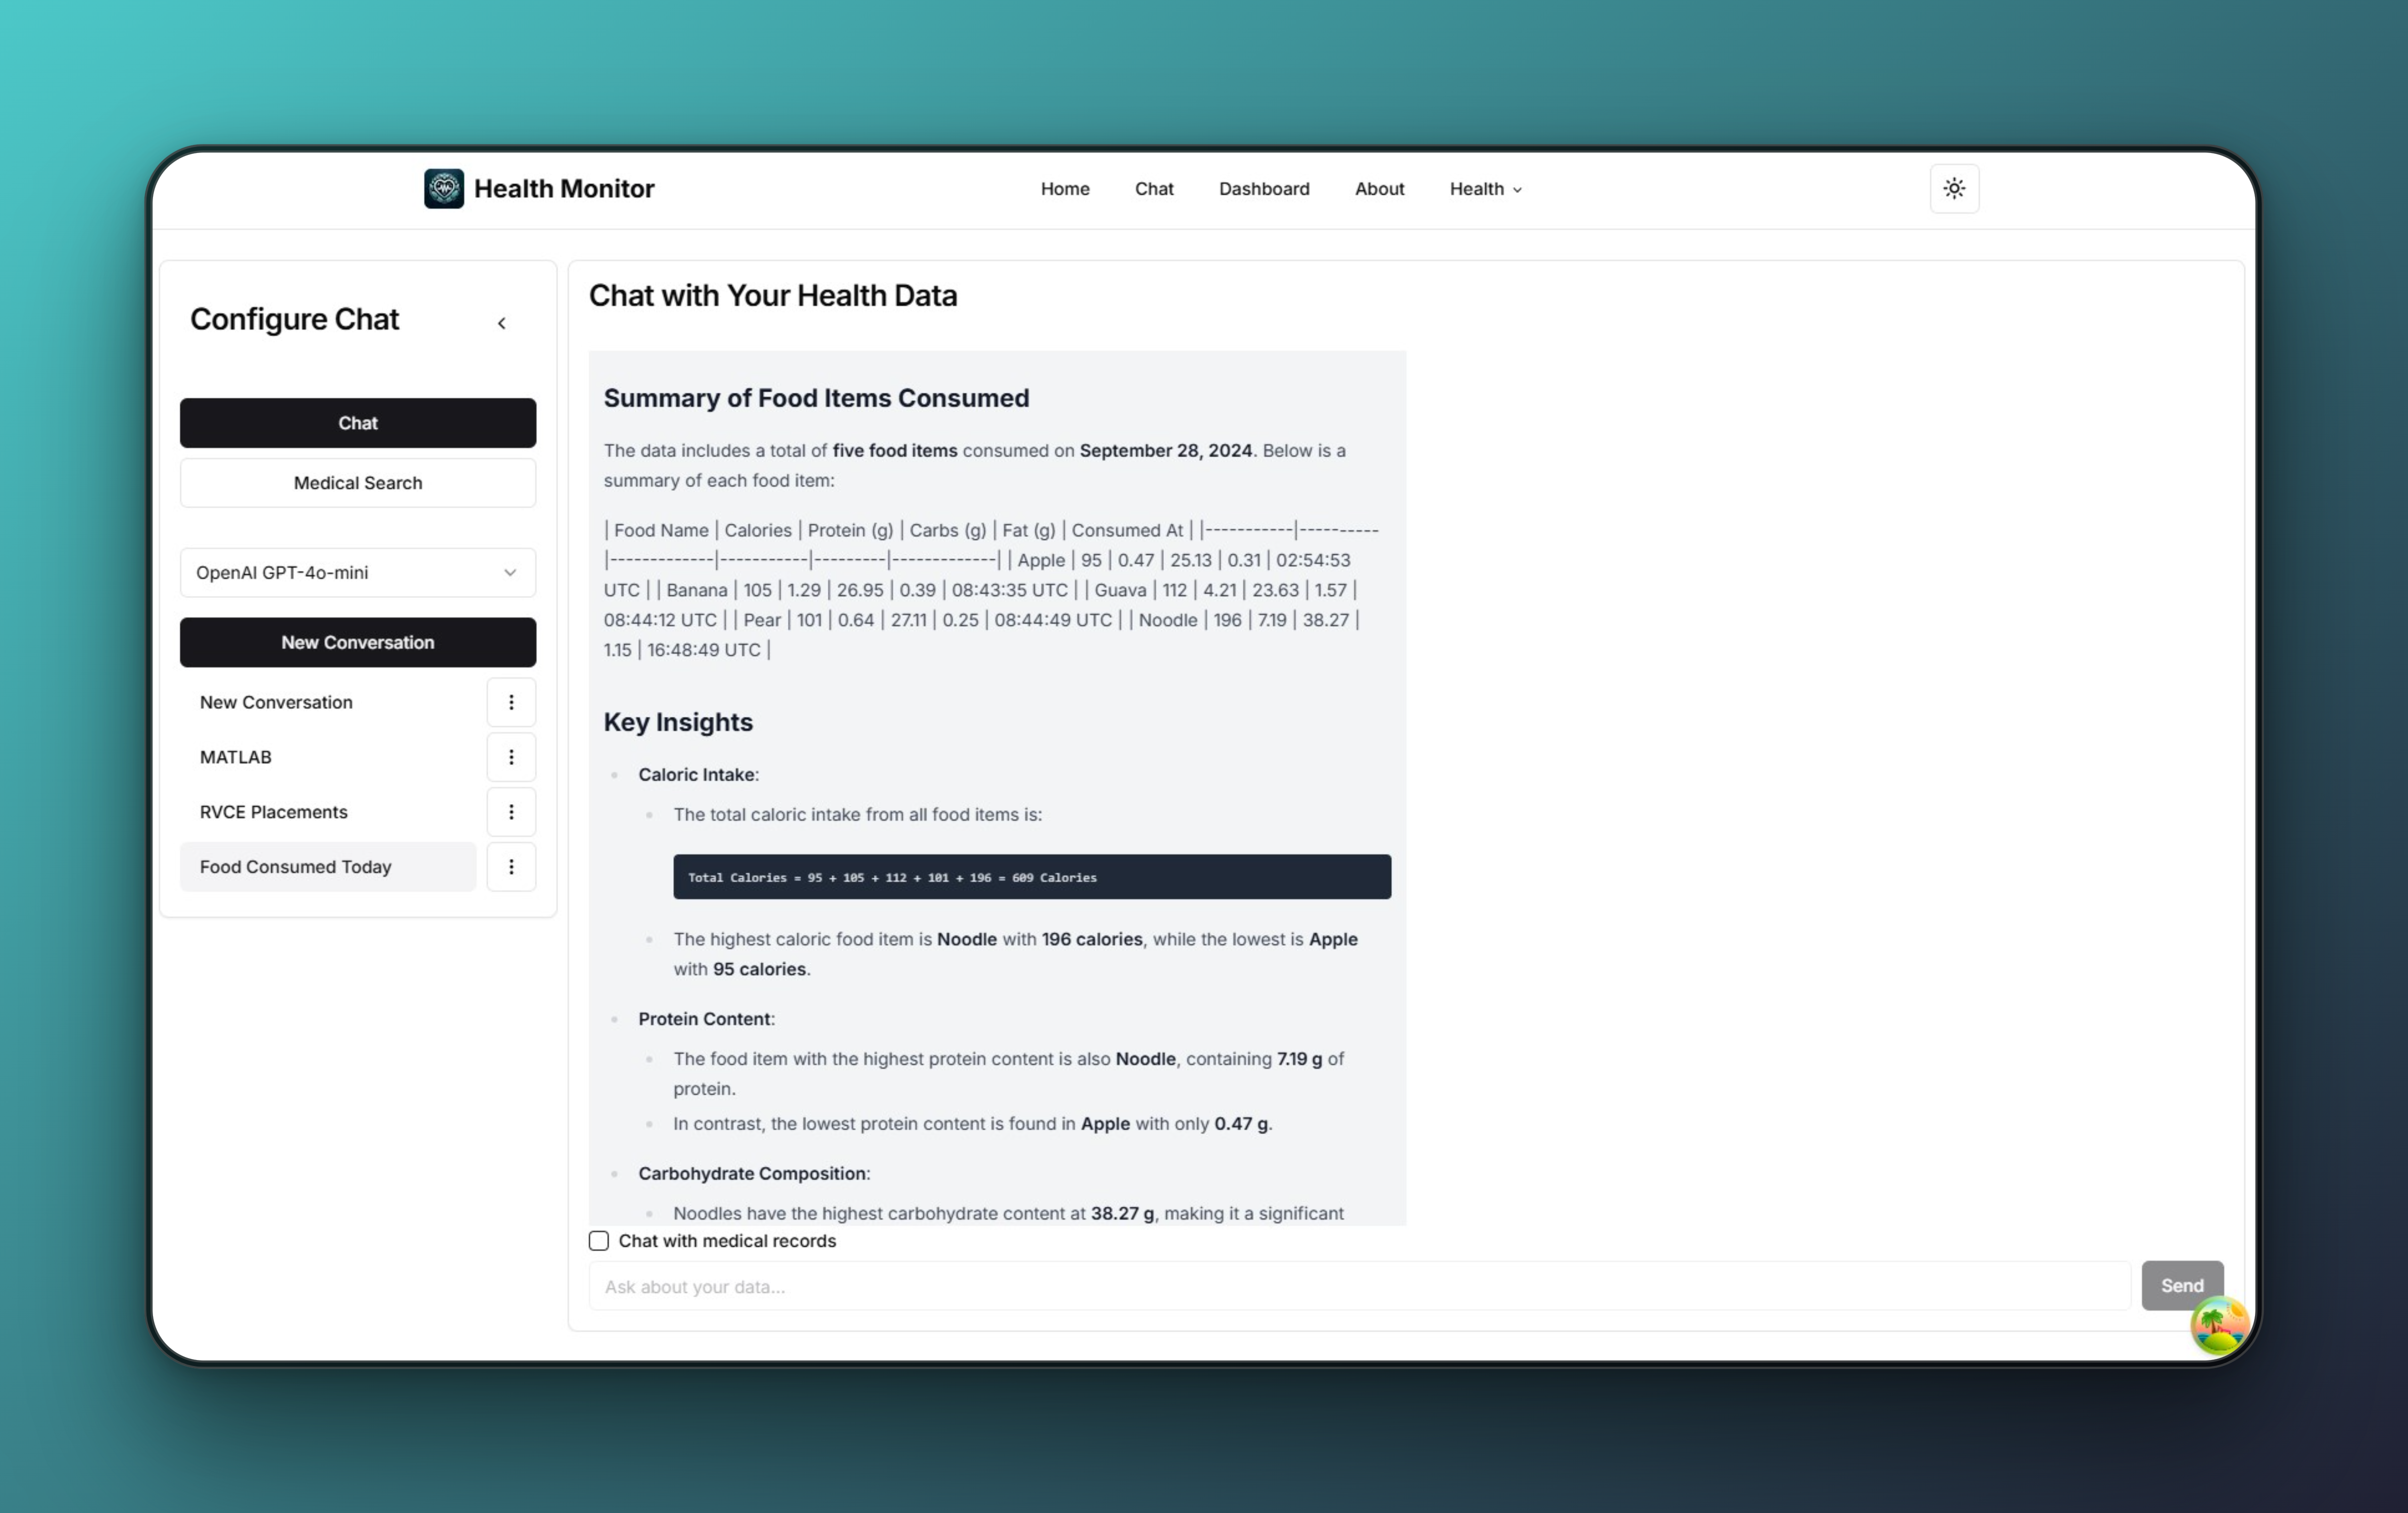
\includegraphics[width=0.8\textwidth]{images/hm-chat-light.png}
    \caption{AI Health Assistant Implementation}
\end{figure}

Chat interface implementation:
\begin{lstlisting}[language=TypeScript, caption=Chat Implementation]
// app/(chat)/chat/ChatPageClient.tsx
export default function ChatPageClient() {
    const [messages, setMessages] = useState<Message[]>([]);
    const [input, setInput] = useState('');

    const handleSubmit = async (e: React.FormEvent) => {
        e.preventDefault();
        if (!input.trim()) return;

        const userMessage = { role: 'user', content: input };
        setMessages(prev => [...prev, userMessage]);
        setInput('');

        try {
            const response = await fetch('/api/chat', {
                method: 'POST',
                body: JSON.stringify({ messages: [...messages, userMessage] })
            });
        } catch (error) {
            console.error('Failed to get response:', error);
        }
    };

    return (
        <div className="chat-container">
            <div className="messages-container">
                {messages.map((msg, idx) => (
                    <MessageComponent key={idx} message={msg} />
                ))}
            </div>
            <form onSubmit={handleSubmit}>
                <input
                    value={input}
                    onChange={(e) => setInput(e.target.value)}
                    placeholder="Ask about your health..."
                />
                <button type="submit">Send</button>
            </form>
        </div>
    );
}
\end{lstlisting}

\section{Data Visualization}
\subsection{Analytics Dashboard}
\begin{figure}[H]
    \centering
    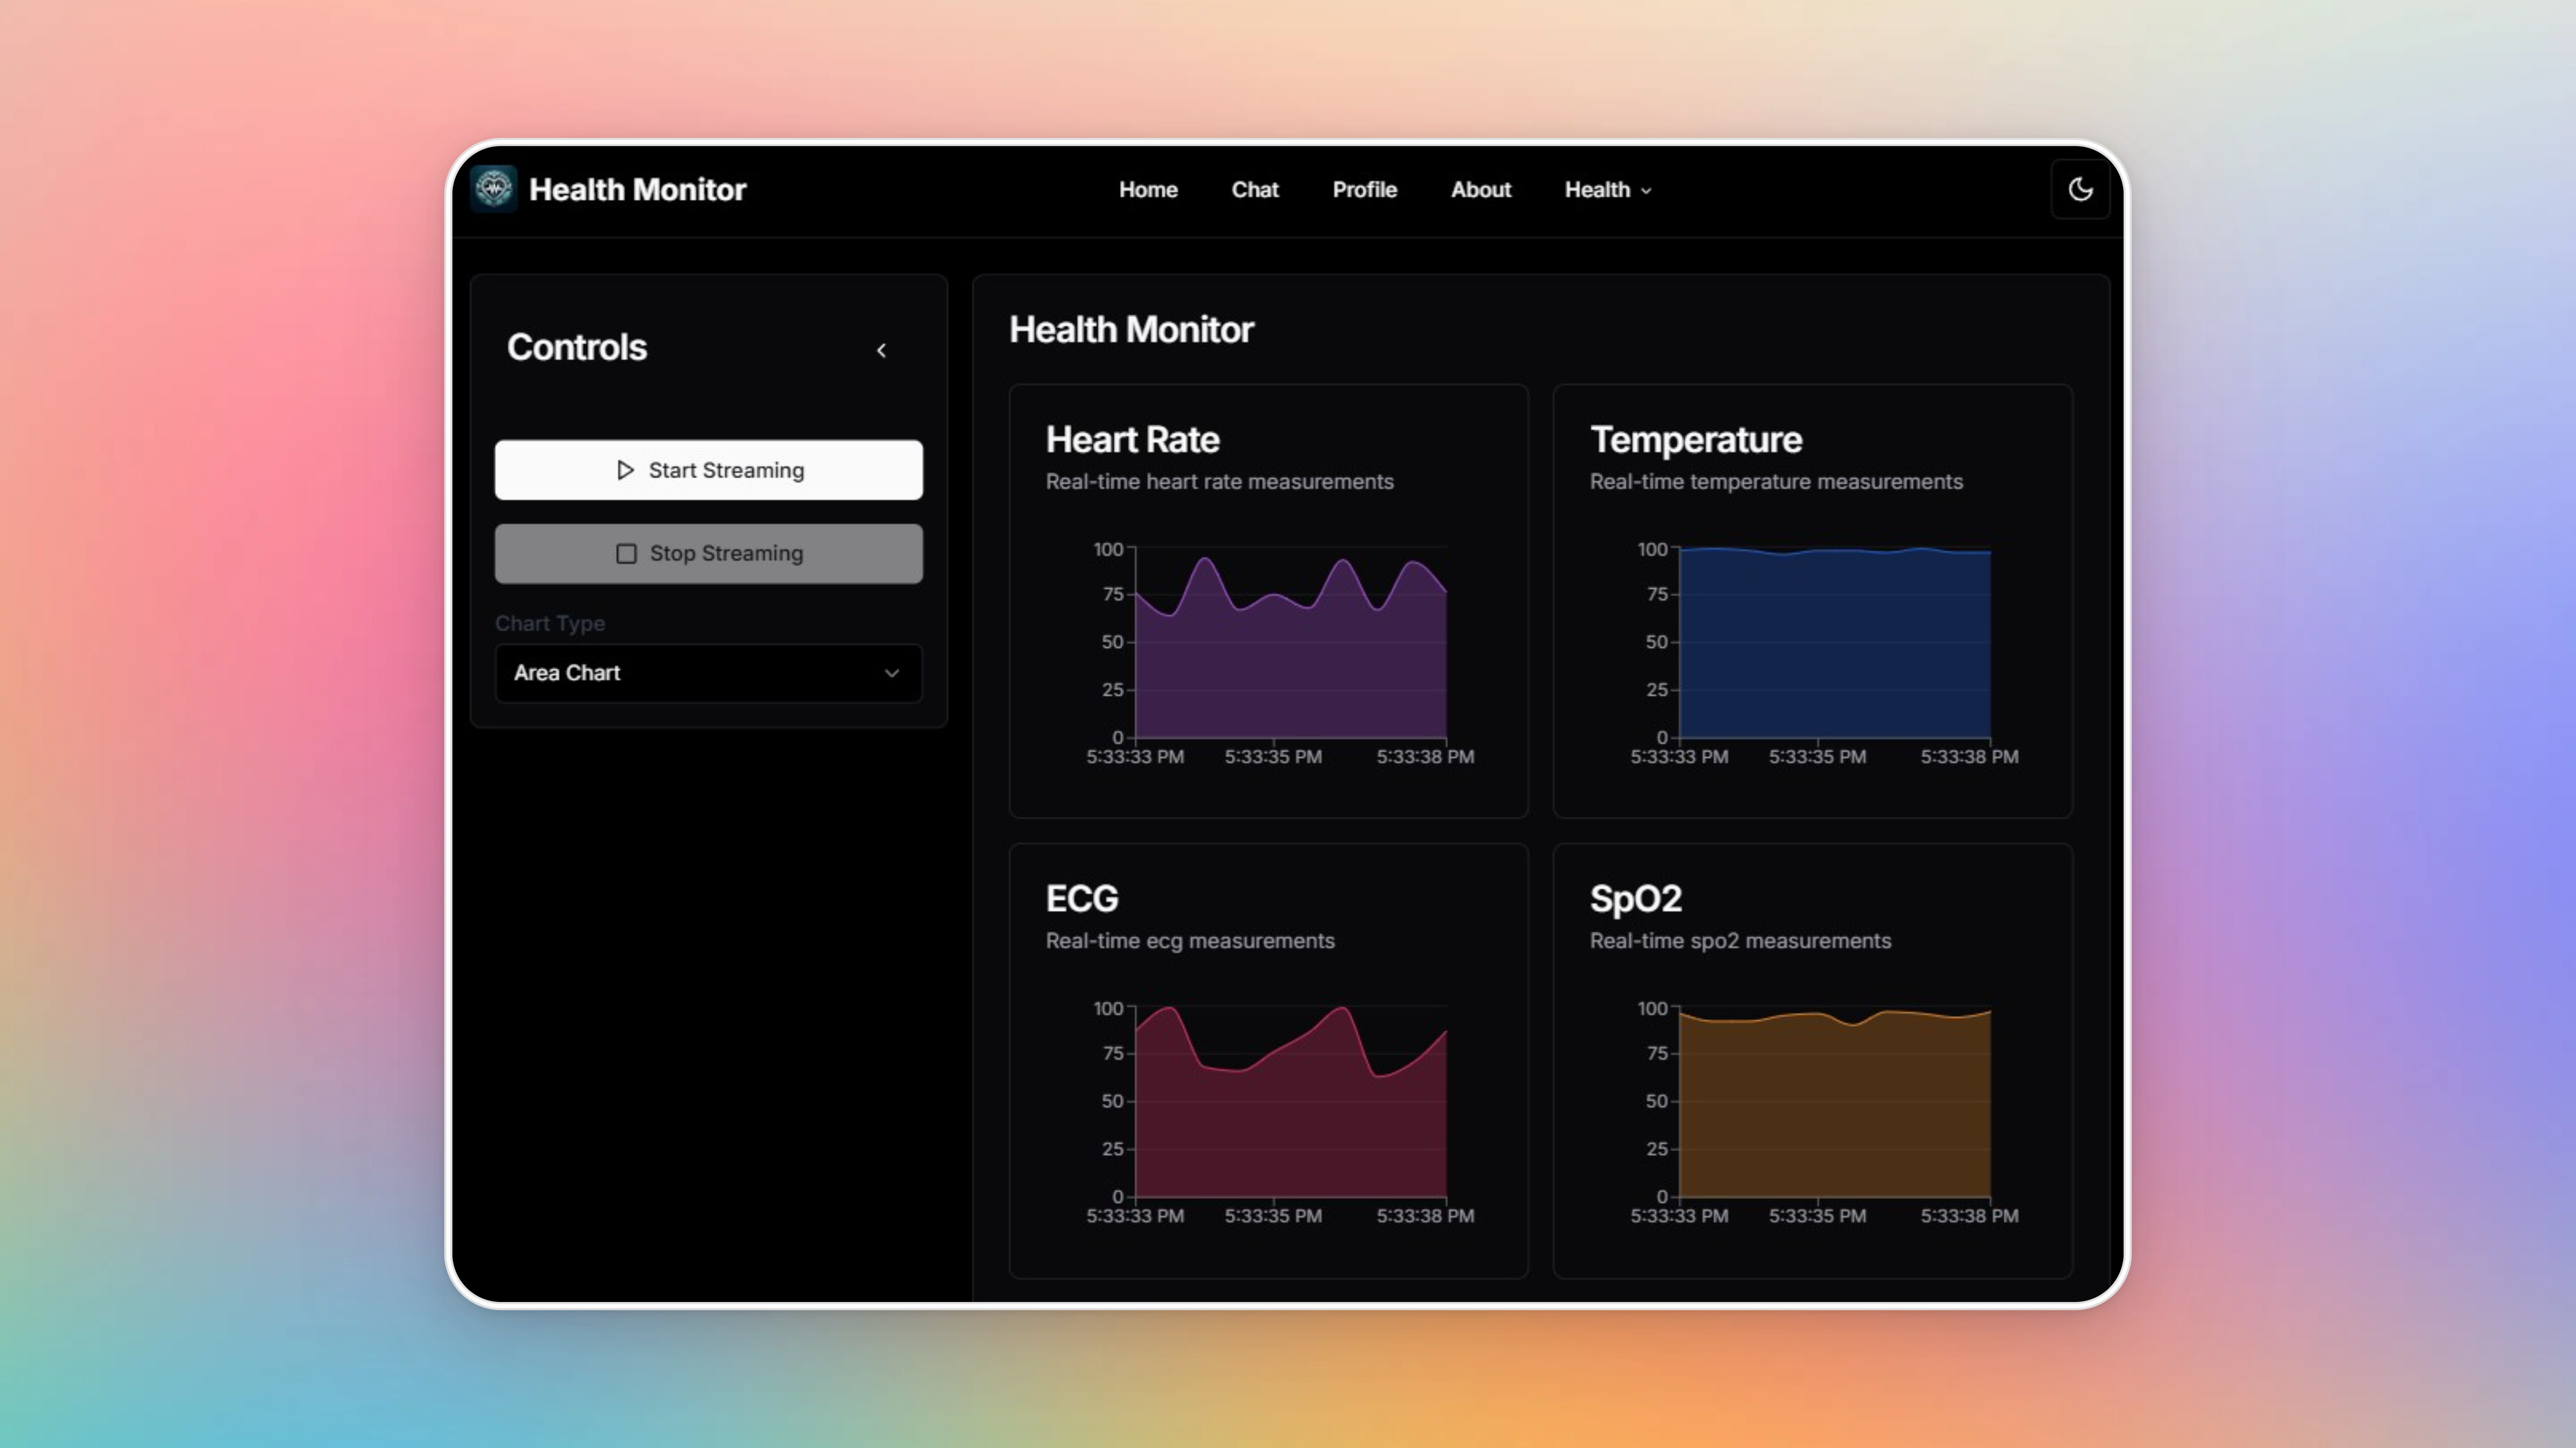
\includegraphics[width=0.8\textwidth]{images/hm-graphs.png}
    \caption{Health Analytics Dashboard}
\end{figure}

\subsection{Record Management}
\begin{figure}[H]
    \centering
    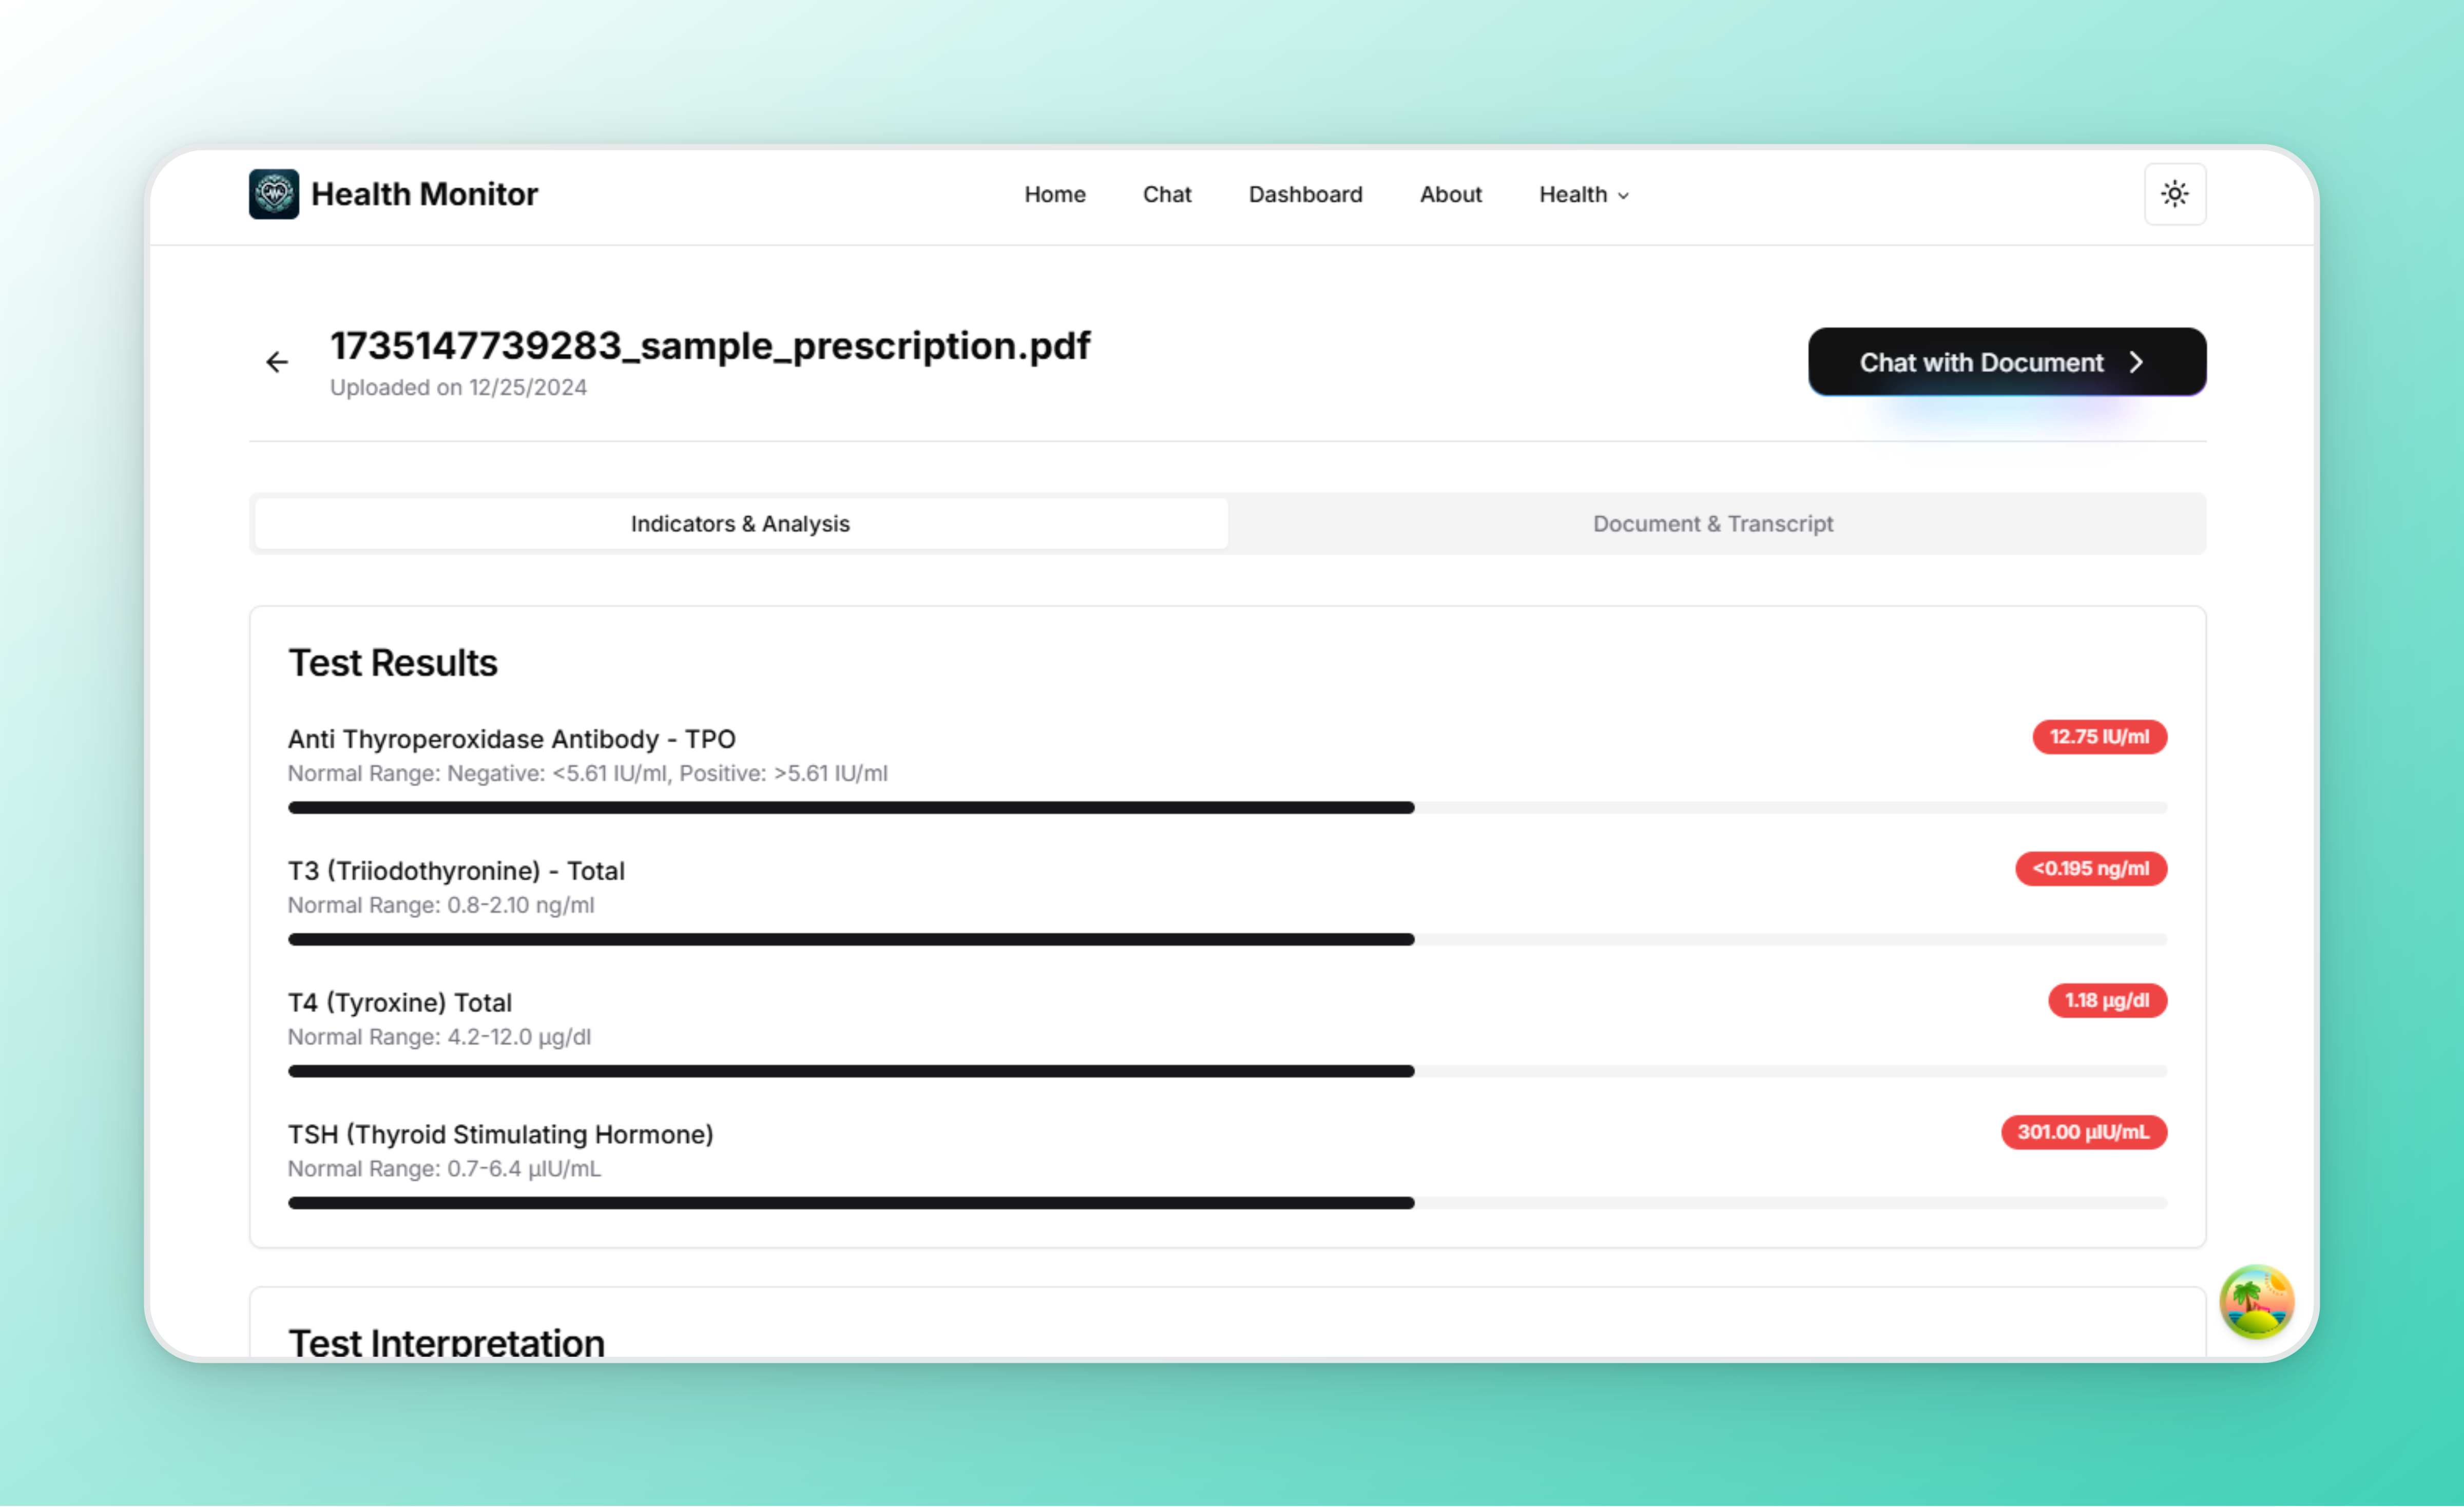
\includegraphics[width=0.8\textwidth]{images/hm-record-analysis.png}
    \caption{Health Record Analysis Interface}
\end{figure}

\section{System Architecture}
\subsection{Activity Monitoring}
\begin{figure}[H]
    \centering
    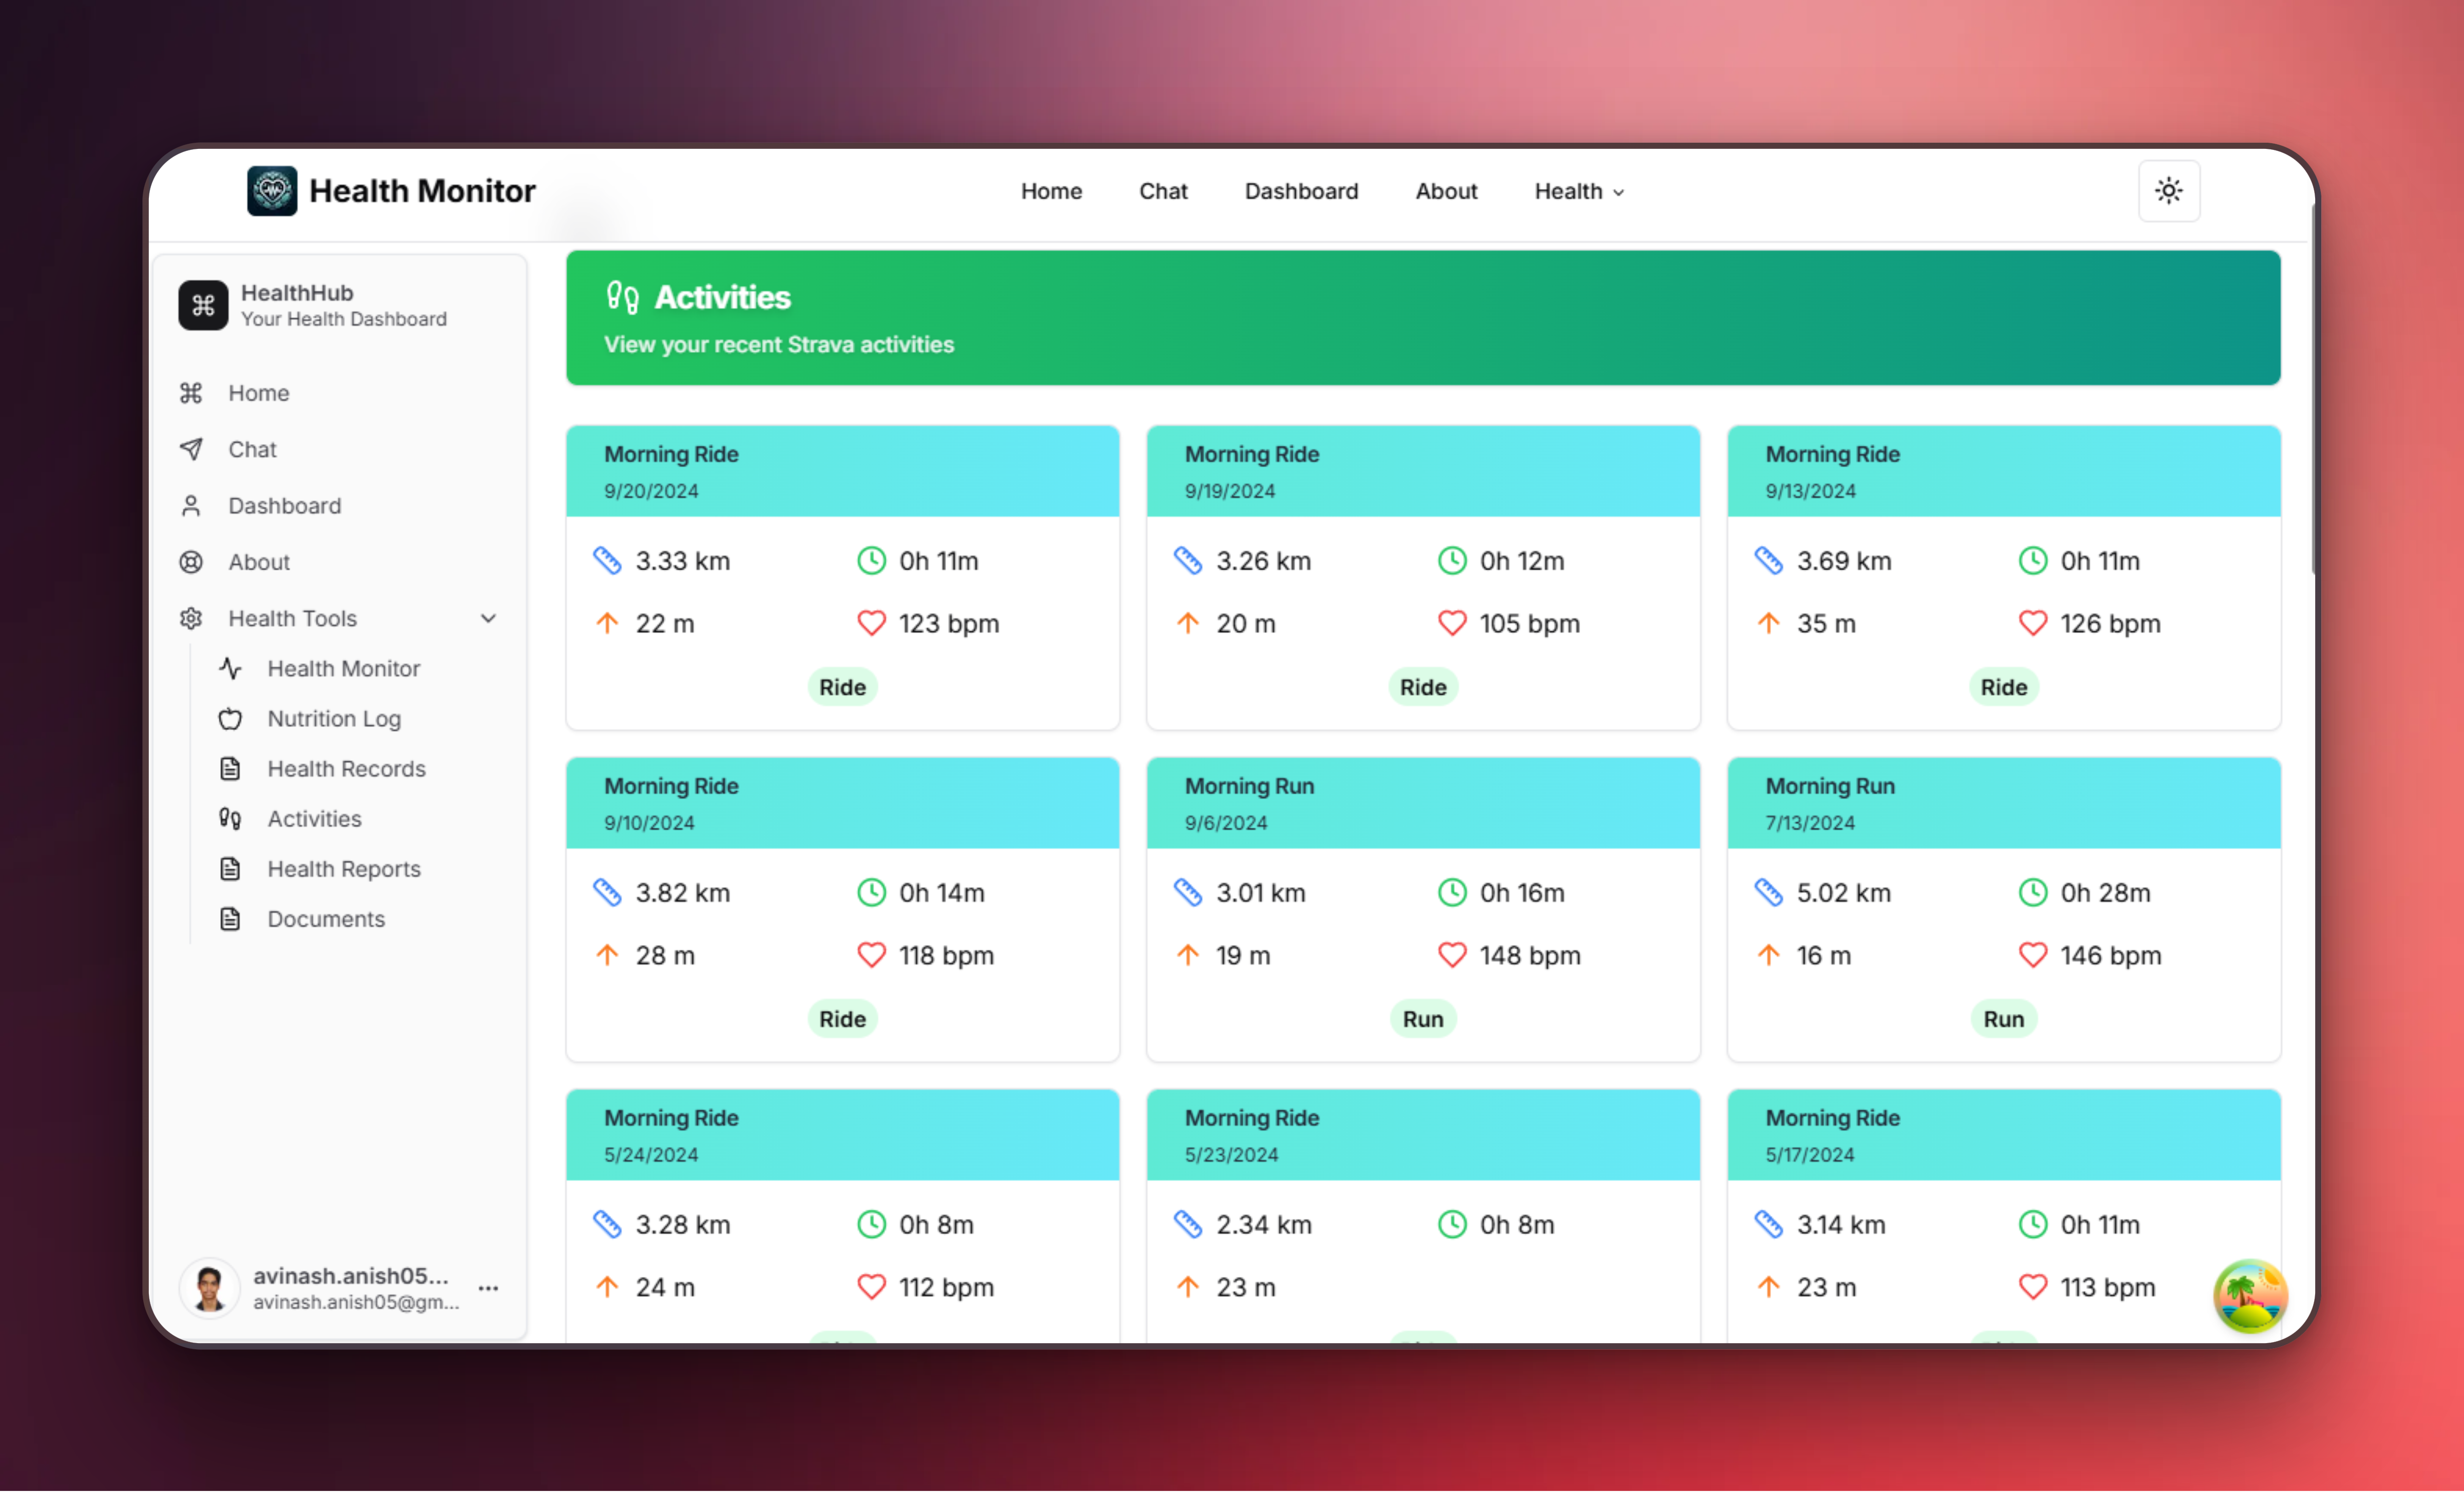
\includegraphics[width=0.8\textwidth]{images/hm-activities.png}
    \caption{Activity Tracking Interface}
\end{figure}

Each interface component was designed with user experience in mind, focusing on clarity, accessibility, and efficient information presentation. The implementation demonstrates the system's capability to handle various aspects of health data management, from real-time monitoring to detailed analysis and AI-assisted interpretation.

\newpage 

% References
\chapter*{REFERENCES}
\addcontentsline{toc}{chapter}{REFERENCES}
\section{References}

[1] M. Alkhalaf, P. Yu, M. Yin, and C. Deng, "Applying generative AI with retrieval-augmented generation to summarize and extract key clinical information from electronic health records," Journal of Biomedical Informatics, p. 104662, 2024.

[2] T. Searle, Z. Ibrahim, J. Teo, and R. J. B. Dobson, "Discharge summary hospital course summarization of inpatient electronic health record text with clinical concept-guided deep pre-trained transformer models," Journal of Biomedical Informatics, p. 104358, 2023.

[3] S. Sai et al., "Generative AI for transformative healthcare: A comprehensive study of emerging models, applications, case studies, and limitations," IEEE Access, vol. 12, pp. 31078-31106, 2024.

[4] S. Reddy, "Generative AI in healthcare: An implementation science-informed translational path on application, integration, and governance," Implementation Science, vol. 19, p. 27, 2024.

[5] P. Zhang and M. N. Kamel Boulos, "Generative AI in medicine and healthcare: Promises, opportunities, and challenges," Future Internet, vol. 15, no. 9, p. 286, 2023.

[6] Leveraging generative AI models for synthetic data generation in healthcare: Balancing research and privacy, in 2023 International Conference on Smart Applications, Communications and Networking (SmartNets), 2023.

[7] W. Saba, S. Wendelken, and J. Shanahan, "Question-answering-based summarization of electronic health records using retrieval-augmented generation," arXiv preprint arXiv:2401.01469, 2024.

[8] Redefining medicine: The power of generative AI in modern healthcare, in 2024 5th International Conference on Smart Electronics and Communication (ICOSEC), 2024.

[9] D. S. W. Ting et al., "Retrieval-augmented generation for large language models and its generalizability in assessing medical fitness," arXiv preprint arXiv:2410.08431, 2024.

[10] L. M. Amugongo et al., "Retrieval-augmented generation for large language models in healthcare: A systematic review," Preprints, 2024.

[11] A. Bora and H. Cuayáhuitl, "Systematic analysis of retrieval-augmented generation-based LLMs for medical chatbot applications," Machine Learning and Knowledge Extraction, vol. 6, pp. 2355–2374, 2024.

[12] E. Albaroudi, T. Mansouri, and A. Alameer, "The intersection of generative AI and healthcare: Addressing challenges to enhance patient care," in 2024 Seventh International Women in Data Science Conference (WiDS PSU), 2024.

[13] Y. Xu, "The investigation of the application of RAG technology in the field of EHR," Science and Technology of Engineering, Chemistry and Environmental Protection, 2024.

[14] C. Troy, S. Sturley, J. M. Alcaraz-Calero, and Q. Wang, "Enabling generative AI to produce SQL statements: A framework for the auto-generation of knowledge based on EBNF context-free grammars," IEEE Access, vol. 11, pp. 123543-123564, 2023.

[15] P. Omrani et al., "Hybrid retrieval-augmented generation approach for LLMs query response enhancement," in 2024 10th International Conference on Web Research (ICWR), 2024.

[16] G. Papanastasiou, N. Dikaios, J. Huang, C. Wang, and G. Yang, "Is attention all you need in medical image analysis? A review," IEEE Journal of Biomedical and Health Informatics, vol. 28, no. 3, pp. 1398-1411, 2024. 

\end{document} 